
\documentclass[t, 11pt]{beamer}
\pdfmapfile{+sansmathaccent.map}
%%% Работа с русским языком
\usepackage{cmap}				
\usepackage{mathtext} 				
\usepackage[T2A]{fontenc}		
\usepackage[utf8]{inputenc}			
\usepackage[russian, english]{babel}	

\usetheme{Montpellier}
\usecolortheme{beaver} % Цветовая схема



%%% Работа с картинками
\usepackage{graphicx}

\usepackage{csquotes}

\hypersetup{				
	colorlinks=true,       	
	linkcolor=blue,          
	citecolor=black,       
	filecolor=magenta,      
	urlcolor=red           
}
%% табличка
\usepackage{booktabs, caption, makecell}
\usepackage{threeparttable}

%% график нормального распределения 
\usepackage{tikz}
\usepackage{xcolor}
\usepackage{pgfplots}
\pgfplotsset{compat=1.7}

%% доп символы
\usepackage{newunicodechar}

\newcommand\Warning{%
	\makebox[1.4em][c]{%
		\makebox[0pt][c]{\raisebox{.1em}{\small!}}%
		\makebox[0pt][c]{\color{red}\Large$\bigtriangleup$}}}%

\newunicodechar{⚠}{\Warning}

\title {Data Transformations}
\subtitle{with dplyr}
\author{Chuvakin Sergey}
\date{\today}
\institute[<<Anthropology>>]{<<School of Advanced Studies>>}

\begin{document}

	
	\frame[plain]{\titlepage}		
	
	\section{Outline}
	
		\begin{frame} 
			\frametitle{\insertsection} 
			\begin{itemize}
				\item Where data can be obtained?
				\item LTE process
				\item Relational database 
				\item What is ID, what is row 
				\item Tidy data 
				\item Cheatsheat  - what should be kept in mind
			\end{itemize}
		\end{frame}
	
	\section{Data Sources}
		\subsection{Where  I can get data?}

	\begin{frame} 
		\frametitle{\insertsection} 
		\framesubtitle{\insertsubsection}
		\begin{itemize}
			\item Self gathering
			\begin{itemize}
				\item Interview 
				\item Survey 
				\item Obsevation 
			\end{itemize}
			\item Public data 
			\begin{itemize}
				\item http://crimestat.ru/
				\item https://rosstat.gov.ru/ (former gks)
				\item WHO data 
				\item World Values Surevey
				\item European Social Survey
			\end{itemize}
			\item Data warehouse, data mart, data lakes - internal statistics of some company 
		\end{itemize}
	
	\end{frame}


	\subsection{ETL processes}
	
	\begin{frame} 
		\frametitle{\insertsection} 
		\framesubtitle{\insertsubsection}
	Extract, Transform, Load - common process in business companies. All the company data are stored in spacial  place named \emph{Database}. Usually enterprises use Structured Query Language (SQL) to store and view the data. The raw data (recently obtained, non transformed) named Data Lake, while Data Warehouse and Data Mart are terms for transformed data (Note: terms maybe different in deferent companies). 
	
	\vspace{1cm}
	
	ETL - process of moving and transforming the data from one source to another. It's essential part data science in enterprise. \href{https://medium.com/@yildirimabdrhm/whats-the-difference-between-oltp-and-olap-bdcafdffb1c3}{See OLAP and OLTP }for better understanding.
	\end{frame}

	 \section{Data sctructure}
	 \subsection{Relational data}
		\begin{frame} 
		\frametitle{\insertsection} 
		\framesubtitle{\insertsubsection}
	\begin{center}
		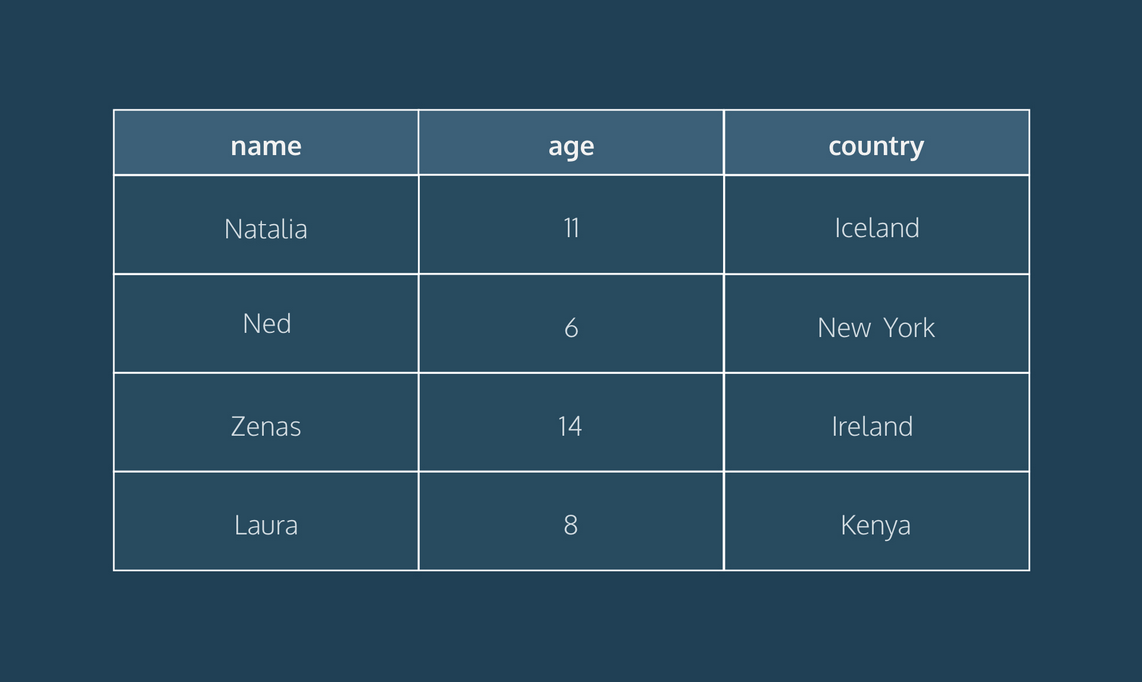
\includegraphics[scale=0.5]{rel_table}
	\end{center}
	\end{frame} 

		\begin{frame} 
		\frametitle{\insertsection} 
		\framesubtitle{\insertsubsection}
	Each row - observation.
	
	Each column - feature. 
	
	Otherwise - it's not relational database. 
	
	\vspace{1cm}
	
	What it gives to social science?
	
	Each row - it's separate vector aka separate person with set of features like sex, age, political preferences et etc. 
	
	\end{frame} 

	\begin{frame} 
	\frametitle{\insertsection} 
	\framesubtitle{\insertsubsection}
 	Each row by default - is unique value, but it's not always true. 
 	\begin{center}
	 	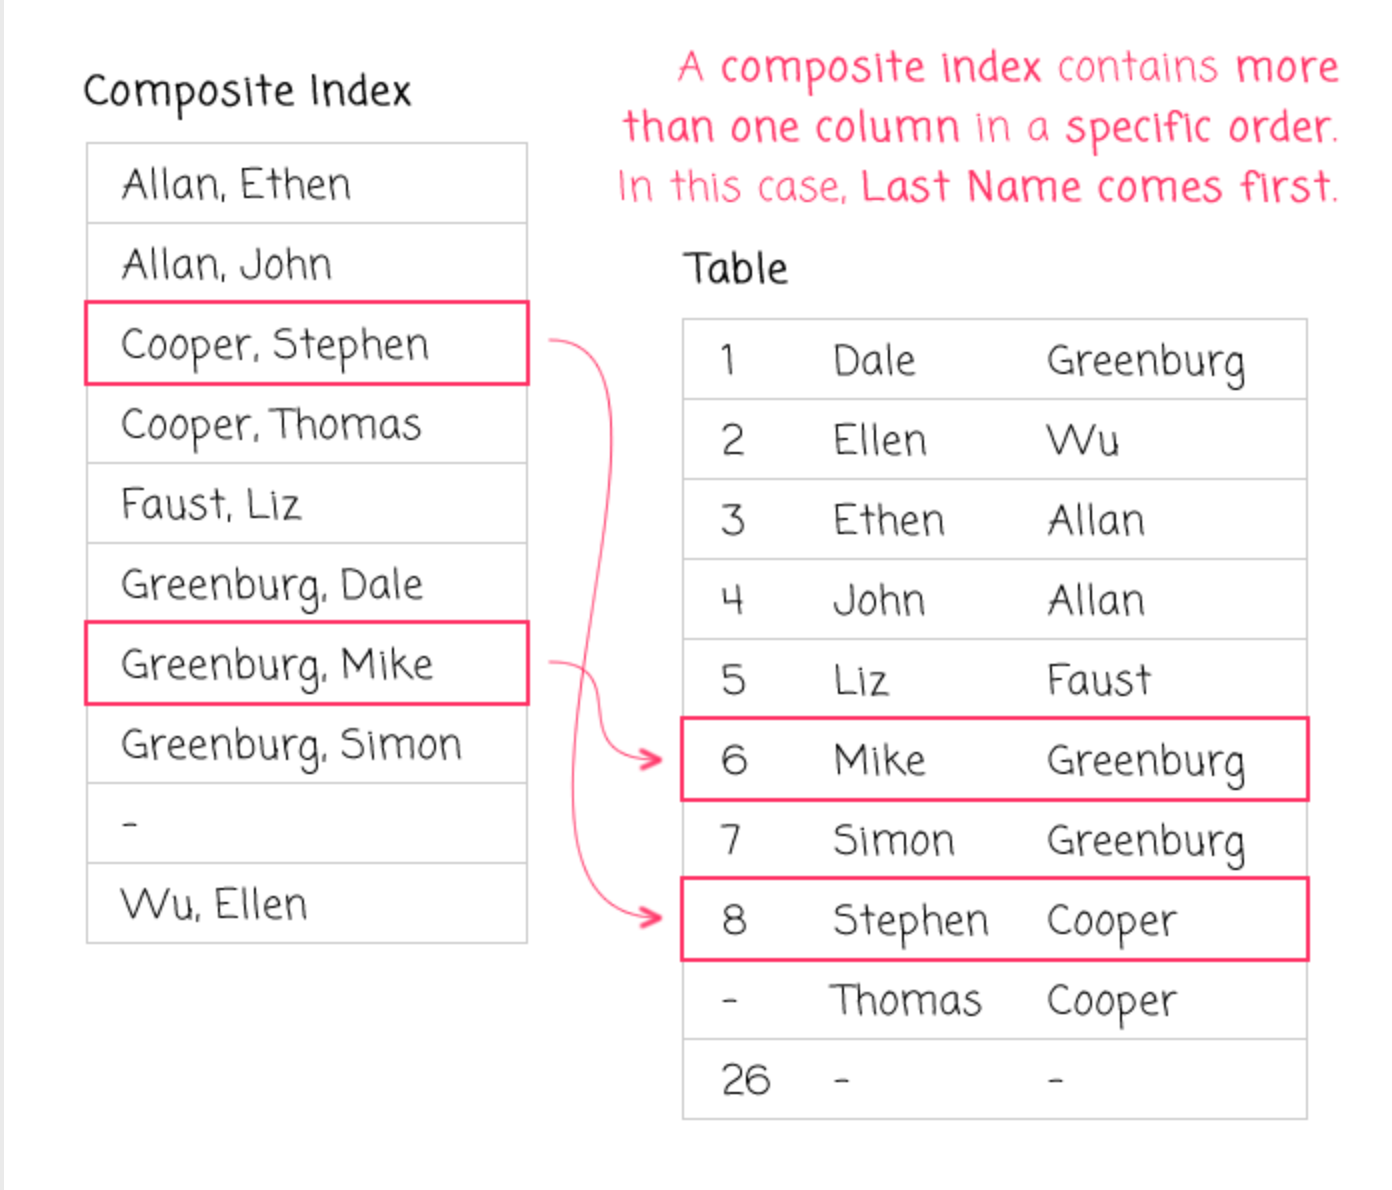
\includegraphics[scale=0.3]{comp_index}
 	\end{center}
	\end{frame} 

	\begin{frame} 
	\frametitle{\insertsection} 
	\framesubtitle{\insertsubsection}
	Sometimes you'll need to group your data to get one observation per row.
	
	 	\begin{center}
		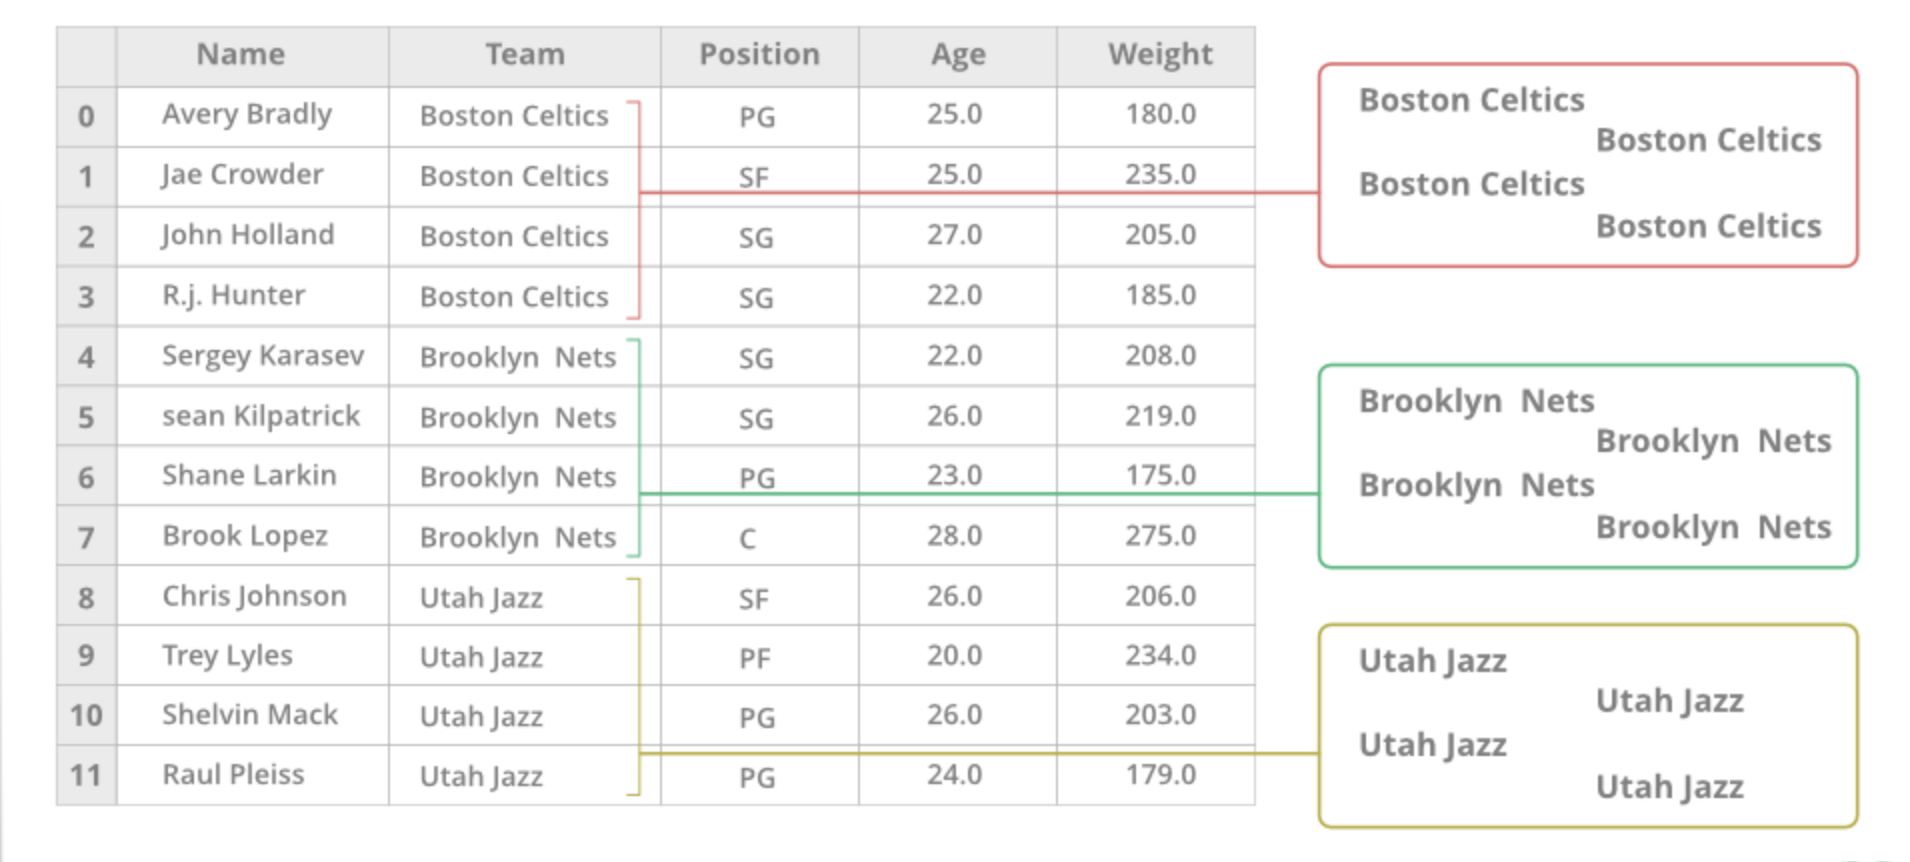
\includegraphics[scale=0.3]{group}
	\end{center}

\end{frame} 

	\subsection{Tidy Data}
	
			\begin{frame} 
		\frametitle{\insertsection} 
		\framesubtitle{\insertsubsection}
		 <<Data tidying>> - making data clean and tidy, ready for analysis and modeling. 
	 
	 Some rules to keep in mind: 
	 
	 \begin{itemize}
	 	 \item One row  should be one obeservaton of your research question
	 	 \item Data should avoid redundancy (data duplicated in several places)
	 	 \item Variables (features) should be only on columns, otherwise to much missings are in data.
	 	\end{itemize}
 	Don't worry if smth is not clear - it becomes transparent with exprience. Obligatory reading in \href{http://vita.had.co.nz/papers/tidy-data.pdf}{English} and in \href{https://habr.com/ru/post/248741/}{Russian}.
 	
	\end{frame}

	\subsection{Cheatsheet}
	\begin{frame} 
	\frametitle{\insertsection} 
	\framesubtitle{\insertsubsection}
 Some things to check before analysis
	\begin{itemize}
		\item Encoding! Does every symbols were read.
		\item Try to avoid spacial symbols like: \$\%$\backslash$* , any slashes, white spaces in columns naming. 
		\item Cyrillic symbols it's mauvais ton because of problems with encodings in diferents OS.
		\item Use sommon formats like csv, tsv or at least xlsx
		\item Try to figure out what means every column in your data.
		\item Explore what is unique ID in your data! 
		\item Explore how your data could be grouped 
		\item Explore basic statistics of your data 
		\item Plot all the variables, discover the data types in your data.
	\end{itemize}
\end{frame}

\end{document}